\documentclass{article}%
\usepackage[T1]{fontenc}%
\usepackage[utf8]{inputenc}%
\usepackage{lmodern}%
\usepackage{textcomp}%
\usepackage{lastpage}%
\usepackage{parskip}%
\usepackage[top=1.2in,bottom=1in,left=0.6in,right=0.6in,headsep=0.8in]{geometry}%
\usepackage{amsmath}%
\usepackage{graphicx}%
\usepackage{needspace}%
\usepackage{color}%
\usepackage{longtable}%
\usepackage{multirow}%
\usepackage[table]{xcolor}%
\usepackage{fancyhdr}%
\usepackage{tabularx}%
%
\definecolor{OsdagGreen}{HTML}{D5DF93}%
\fancypagestyle{header}{ 
\renewcommand{\headrulewidth}{0pt}%
\renewcommand{\footrulewidth}{0pt}%
\fancyhead{ 
}%
\fancyfoot{ 
}%
\fancyhead[C]{ 
\begin{tabularx}{\textwidth}{|l|p{6cm}|l|X|}%
\hline%
\rowcolor{OsdagGreen}%
Company Name&LoremIpsum&Project Title&Fossee\\%
\hline%
\rowcolor{OsdagGreen}%
Group/Team Name&LoremIpsum&Subtitle&\\%
\hline%
\rowcolor{OsdagGreen}%
Designer&LoremIpsum&Job Number&123\\%
\hline%
\rowcolor{OsdagGreen}%
Date&18 /05 /2020&Client&LoremIpsum\\%
\hline%
\end{tabularx}
}%
\fancyfoot[R]{ 
Page \thepage\ of \pageref{LastPage}
}
}%
%
\begin{document}%
\normalsize%
\pagestyle{header}%
\section{Input Parameters}%
\label{sec:InputParameters}%
\renewcommand{\arraystretch}{1.2}%
\begin{longtable}{|p{5cm}|p{2cm}|p{2cm}|p{2cm}|p{5cm}|}%
\hline%
\hline%
\multicolumn{3}{|c|}{Module}&\multicolumn{2}{|c|}{Beam Coverplate  Weld Connection}\\%
\hline%
\hline%
\multicolumn{3}{|c|}{MainModule}&\multicolumn{2}{|c|}{Moment Connection}\\%
\hline%
\hline%
\multicolumn{3}{|c|}{Moment(kNm)*}&\multicolumn{2}{|c|}{10.0}\\%
\hline%
\hline%
\multicolumn{3}{|c|}{Shear(kN)*}&\multicolumn{2}{|c|}{10.0}\\%
\hline%
\hline%
\multicolumn{3}{|c|}{Axial (kN) *}&\multicolumn{2}{|c|}{10.0}\\%
\hline%
\hline%
\multicolumn{5}{|c|}{\textbf{Section}}\\%
\hline%
\hline%
\multirow{13}{*}{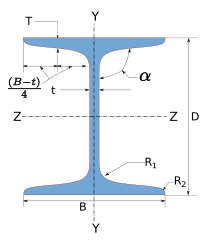
\includegraphics[width=5cm,height=5cm]{C:/Users/nitin/Pictures/Saved Pictures/Osdag3/ResourceFiles/images/ISection.png}}&\multicolumn{2}{|c|}{Beam Section *}&\multicolumn{2}{|c|}{NPB 270x135x30.7}\\%
\cline{2%
-%
5}%
&\multicolumn{2}{|c|}{Material *}&\multicolumn{2}{|c|}{E 250 (Fe 410 W)A}\\%
\cline{2%
-%
5}%
&\multicolumn{2}{|c|}{Ultimate strength, fu (MPa)}&\multicolumn{2}{|c|}{410}\\%
\cline{2%
-%
5}%
&\multicolumn{2}{|c|}{Yield Strength , fy (MPa)}&\multicolumn{2}{|c|}{250}\\%
\cline{2%
-%
5}%
&Mass&30.73&Iz(mm4)&49173000.0\\%
\cline{2%
-%
5}%
&Area(mm2) {-} A&3910.0&Iy(mm4)&3574200.0\\%
\cline{2%
-%
5}%
&D(mm)&267.0&rz(mm)&112.10000000000001\\%
\cline{2%
-%
5}%
&B(mm)&135.0&ry(mm)&30.2\\%
\cline{2%
-%
5}%
&t(mm)&5.5&Zz(mm3)&368340.0\\%
\cline{2%
-%
5}%
&T(mm)&8.7&Zy(mm3)&52950.0\\%
\cline{2%
-%
5}%
&FlangeSlope&90&Zpz(mm3)&412490.0\\%
\cline{2%
-%
5}%
&R1(mm)&1.5&Zpy(mm3)&52950.0\\%
\cline{2%
-%
5}%
&R2(mm)&0.0&&\\%
\cline{2%
-%
5}%
\hline%
\multicolumn{5}{|c|}{\textbf{Weld Details}}\\%
\hline%
\hline%
\multicolumn{3}{|c|}{Weld Type}&\multicolumn{2}{|c|}{Fillet}\\%
\hline%
\hline%
\multicolumn{3}{|c|}{Type of weld fabrication}&\multicolumn{2}{|c|}{Shop Weld}\\%
\hline%
\hline%
\multicolumn{3}{|c|}{Material grade overwrite (MPa) Fu}&\multicolumn{2}{|c|}{410.0}\\%
\hline%
\end{longtable}

%
\Needspace{10\baselineskip}%
\newpage%
\section{Design Checks}%
\label{sec:DesignChecks}%
\subsection{Member Capacity}%
\label{subsec:MemberCapacity}%
\renewcommand{\arraystretch}{1.2}%
\begin{longtable}{|p{4cm}|p{5cm}|p{5.5cm}|p{1.5cm}|}%
\hline%
\rowcolor{OsdagGreen}%
Check&Required&Provided&Remarks\\%
\hline%
\endhead%
\hline%
Axial Capacity Ac (kN)&&$\begin{aligned} Ac &=\frac{A*f_y}{\gamma_{m0} *1000}\\ &=\frac{3910.0*250}{1.1* 1000}\\ &=888.64\end{aligned}$&\\%
\hline%
Shear Capacity Sc (kN)&&$\begin{aligned} S_c &= \frac{A_v*f_y}{\sqrt{3}*\gamma_{mo} *1000}\\ &=\frac{249.6*5.5*250}{\sqrt{3}*1.1 *1000}\\ &=180.13327999999998\end{aligned}$&\\%
\hline%
Plastic Moment Capacity Pmc (kNm)&&$\begin{aligned} Pmc &= \frac{\beta_b * Z_p *fy}{\gamma_{mo} * 1000000}\\ &=\frac{1*85663*250}{1.1 * 1000000}\\ &=19.47\end{aligned}$&\\%
\hline%
Moment Deformation Criteria Mdc (kNm)&&$\begin{aligned} Mdc &= \frac{1.5 *Z_e *fy}{1.1}\\ &= \frac{1.5 *368340.0*250}{1.1}\\ &= 125.57\end{aligned}$&\\%
\hline%
Moment Capacity Mc (kNm)&&$\begin{aligned} M_c &= min(Pmc,Mdc)\\ &=min(19.47,125.57)\\ &=19.47\end{aligned}$&\\%
\hline%
\end{longtable}

%
\newpage%
\subsection{Load Consideration}%
\label{subsec:LoadConsideration}%
\renewcommand{\arraystretch}{1.2}%
\begin{longtable}{|p{4cm}|p{5cm}|p{5.5cm}|p{1.5cm}|}%
\hline%
\rowcolor{OsdagGreen}%
Check&Required&Provided&Remarks\\%
\hline%
\endhead%
\hline%
Axial Load Au (kN)&$\begin{aligned} Ac_{min} &= 0.3 * A_c\\ &= 0.3 *888.64\\ &=266.59\end{aligned}$&$\begin{aligned} Au &= max(A,Ac_{min} )\\ &= max( 10.0,266.59)\\ &=266.59\end{aligned}$&Pass\\%
\hline%
Shear Load Vu (kN)&$\begin{aligned} Sc_{min} &= 0.6 * A_c\\ &= 0.6 *180.13\\ &=108.08\end{aligned}$&$\begin{aligned} Vu &= max(V,Vc_{min})\\ &=  max(10.0,108.08)\\ &=108.08\end{aligned}$&Pass\\%
\hline%
Moment Load Mu (kNm)&$\begin{aligned} Mc_{min} &= 0.5 * M_c\\ &= 0.5 *19.47\\ &=9.73\end{aligned}$&$\begin{aligned} Mu &= max(M,Mc_{min} )\\ &= max(10.0,9.73)\\ &=10.0\end{aligned}$&Pass\\%
\hline%
Forces Carried by Web&&$\begin{aligned}A_w &= Axial~ force~ in~ web  \\   &= \frac{(D- 2*T)*t* Au }{A} \\ &= \frac{(267.0- 2*8.7)*5.5*266.59 }{3910.0} \\ &=93.6\\ M_w &= Moment ~in ~web  \\  &= \frac{Z_w * Mu}{Z} \\ &= \frac{85663 * 10.0}{412490.0} \\ &=2.08\end{aligned}$&\\%
\hline%
Forces Carried by Flange&&$\begin{aligned} A_f&= Axial~force~ in ~flange  \\ &= \frac{Au * B *T}{A} \\ &= \frac{266.59 * 135.0*8.7}{3910.0} \\ &=80.08\\ M_f& =Moment~ in~ flange \\  & = Mu-M_w\\ &= 10.0-2.08\\ &=7.92\\  F_f& =flange~force  \\ & = \frac{M_f *1000}{D-T} + A_f \\ &= \frac{7.92}{267.0-8.7} +80.08 \\ &=110.75\end{aligned}$&\\%
\hline%
\end{longtable}

%
\newpage%
\subsection{Weld Design Checks}%
\label{subsec:WeldDesignChecks}%
\renewcommand{\arraystretch}{1.2}%
\begin{longtable}{|p{4cm}|p{5cm}|p{5.5cm}|p{1.5cm}|}%
\hline%
\rowcolor{OsdagGreen}%
Check&Required&Provided&Remarks\\%
\hline%
\endhead%
\hline%
Min Weld Size (mm)&$\begin{aligned} &Thickness~of~Thicker~part\\ \noindent &=max(8.7,14.0)\\ &=14.0\\ &IS800:2007~cl.10.5.2.3~Table 21,\\  &t_{w_{min}}=5\end{aligned}$&7&Pass\\%
\hline%
Max Weld Size (mm)&$\begin{aligned} & Thickness~of~Thinner~part\\ &=Min(8.7,14.0)=8.7\\ &t_{w_{max}} =8.7\end{aligned}$&7&Pass\\%
\hline%
Flange Weld Strength (N/mm)&$\begin{aligned} Stress &= \frac{F_f*1000}{F_{rl}}\\  &= \frac{110.75*1000}{391}\\ &= 283.2588987614436\end{aligned}$&927.92&Pass\\%
\hline%
\end{longtable}

%
\newpage%
\subsection{Flange Plate Check}%
\label{subsec:FlangePlateCheck}%
\renewcommand{\arraystretch}{1.2}%
\begin{longtable}{|p{4cm}|p{6cm}|p{5.5cm}|p{1.5cm}|}%
\hline%
\rowcolor{OsdagGreen}%
Check&Required&Provided&Remarks\\%
\hline%
\endhead%
\hline%
Min. Plate Height (mm)&50&$\begin{aligned} b_{fp} &= {B - 2*sp} \\ &= {135.0 - 2 * 15} \\ &=105\end{aligned}$&Pass\\%
\hline%
Max. Plate Height (mm)&$\begin{aligned} b_{fp} &= {B - 2*sp} \\ &= {135.0 - 2 * 15} \\ &=105\end{aligned}$&105&Pass\\%
\hline%
Min. Plate Length (mm)&105&$\begin{aligned} l_{fp} & = [2*(l_{w} + 2*s) + g]\\ &= [2*(1502*7) +10.0]\\ &=340\end{aligned}$&Pass\\%
\hline%
\end{longtable}

%
\Needspace{10\baselineskip}%
\newpage%
\section{3D View}%
\label{sec:3DView}%


\begin{figure}[h!]%
\centering%
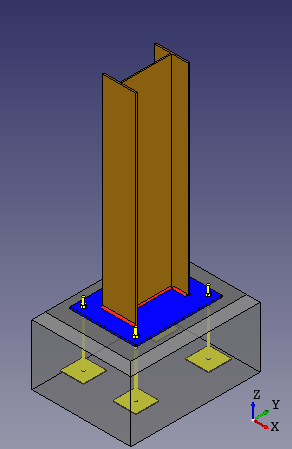
\includegraphics[width=\linewidth]{C:/Users/nitin/Pictures/Saved Pictures/Osdag3/ResourceFiles/images/3d.png}%
\caption{3D View}%
\end{figure}

%
\end{document}